% !TEX root = ../ac_paper.tex

\section{Breadth first search}

% Sketch of the section: We use search algorithm to get a baseline on results. We call it breadth-first search. It is able to solve less than half of the presentations we considered. We will use these presentations to generate dataset for each of the techniques used in the next two sections: for embeddings, we generate text dataset, for reinforcement learning, these states are the initial states of a Markov Decision Process. 

\fixme{Made search space finite. Perhaps this could be discussed in the previous section. Justify the BFS name.}


We use the algorithm presented in Algorithm \autoref{alg:bfs} to classify these examples as solved or unsolved.
For each presentation $R_0$, we start with a heap $H$ and a set $S$; each of them containing only $R_0$.
The heap $H$ is ordered by a tuple $(n, m)$ where $n$ is the total length of a presentation and $m$ is the length of the sequence of AC moves connecting a presentation and $R_0$.
We put a hard cutoff of $10^6$ on the number of nodes of the tree. With this choice, we found that each example took 1-2 minutes to process.
For 1190 presentations, this amounted to approximately 20 hours. \fixme{CPU Time?}
If the algorithm finds the trivial presentation, we consider the starting presentation $R_0$ 'BFS-easy'; else, we consider it a 'BFS-hard' example.
The sequence we first encounter depends on the choice of sequence of AC moves in the for loop.
What is that sequence in our case?
Isn't S a set instead of a list? Specify what Actions, H, $N_f$ mean in our case.
Why should this algorithm be called BFS?

\begin{algorithm}
	\caption{Search algorithm}\label{alg:bfs}
	\begin{algorithmic}
		\State $H \gets R_0$ \Comment{Initialize the heap of presentations with $R_0$.}
		\State $S \gets R_0$ \Comment{Initialize the set of seen presentations with $R_0$.}

		\While{$\text{len}(S) < 10^6$} \Comment{While number of nodes in $S$ is less than $N$.}
		\State $R \gets H[0]$ \Comment{Pop the top element of the heap.}
		\For{$A \in \text{AC Moves}$}
		\State $RA \gets A \cdot R$ \Comment{Act on $R$ by $A$.}
		\If{RA is trivial}
		\Return{True}
		\Else{ $RA \notin S$}
		\State $S \gets RA$
		\State $H \gets RA$ \Comment{Add $RA$ to $H$ keeping the heap invariant.}

		\EndIf
		\EndFor
		\EndWhile
	\end{algorithmic}
\end{algorithm}

The number of BFS-hard examples increases as a function of $n$.
(See \autoref{fig:hist_vs_n}.)
The distributions of BFS-easy and BFS-hard as a function of the total length of a presentation are also given in \autoref{fig:hist_vs_length}.

\begin{figure}
	\centering
	\begin{subfigure}[b]{0.5\textwidth}
		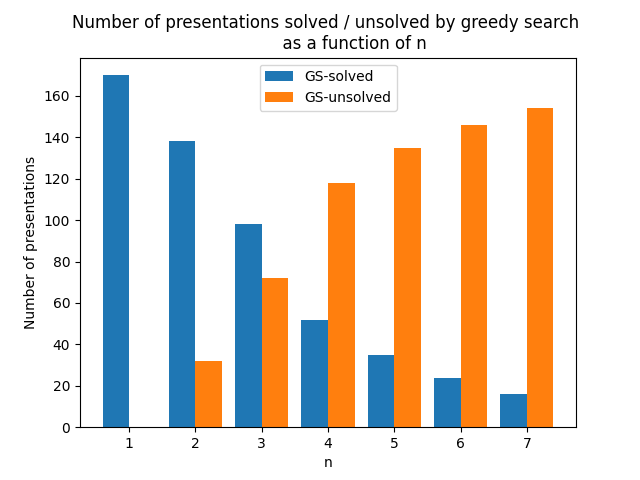
\includegraphics[width=\textwidth]{fig/hist_vs_n.png}
		\caption{Distribution versus $n$}
		\label{fig:hist_vs_n}
	\end{subfigure}%
	%add desired spacing between images, e. g. ~, \quad, \qquad etc.
	%(or a blank line to force the subfigure onto a new line)
	\begin{subfigure}[b]{0.5\textwidth}
		\centering
		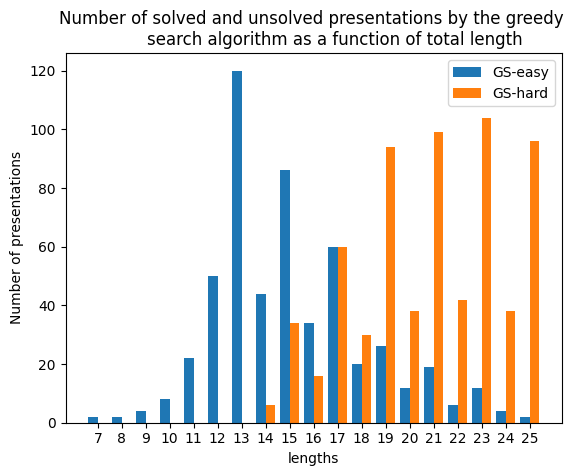
\includegraphics[width=\textwidth]{fig/hist_vs_lengths.png}
		\caption{Distribution versus total length}
		\label{fig:hist_vs_length}
	\end{subfigure}
	\caption{Number of presentations}\label{fig:miller_schupp_statistics}
\end{figure}